\section{Methodology}

\begin{figure}[t]
    \centering
    \includegraphics[width=\linewidth]{figures/03_introduction/BlockDiagram.png}
    \caption[Project's Block diagram]{\footnotesize{Block diagram of the project}}
    \label{fig:block_diagram}
\end{figure}

{
    This section offers an in-depth exploration of the research framework, 
    starting with a high-level overview of the project's key components. 
    The research project encompasses three core components:
}

\begin{itemize}
    \item {
        \textbf{Detection}: 
        This component focuses on the initial step of locating ants within video frames. 
        It plays a fundamental role in the subsequent stages of re-identification and tracking. 
        It requires a reasonable amount of labeled image data.
    }
    \item {
        \textbf{Re-identification (ReID)}: 
        ReID is the aspect of the research involving the identification of previously detected ants through visual features. 
        It aims to associate ants with their unique visual identities as they move throughout the video, 
        highlighting the case where ants disappear for a long period. 
        It demands a substantial number of labeled identities for a significant volume of cropped detection images.
    }
    \item {
        \textbf{Tracking}:
        The tracking component is the culmination of the research framework, 
        combining detection and re-identification to trace the ants trajectories across time. 
        The contemplated approches need few labeled video data to test its performance.
    }
\end{itemize}

{
    This high-level system architecture, as well as the requiered resources, inputs and outputs, is depicted in the Figure \ref{fig:block_diagram}. 
    Additionally, the three components have their own performance measurments and metrics.
}

\begin{samepage}

    {
        Following the research framework and system overview, the methodology section is structured into five subsections:
    }
    
    \nopagebreak

    \begin{enumerate}
        \item {
            \textbf{Data and Datasets}: 
            This subsection details the gathered data and the methodologies used for labeling the ants for the different tasks.
        }
        \item {
            \textbf{Metrics}:
            This subsection comprehensively presents the performance metrics and criteria used to assess the performance of the detection (mAP), re-identification (rank-N), and tracking models (HOTA).
        }
        \item {
            \textbf{Detection model}:
            This subsection explores the specifics of both an initial deductive model and the chosen detection model, including their implementation, training processes (for the chosen model), and key considerations.
        }
        \item {
            \textbf{Appearance model}:
            This subsection delves into the specificities of the appearance model including the implementation, training process and key considerations.
        }
        \item {
            \textbf{Tracking}:
            Finally, we explore the tracking component, were detection, re-identification, 
            motion estimation and location metrics are integrated into a cohesive system for continuous multiple ants tracking.
        }
    \end{enumerate}
\end{samepage}

{
    Each subsection corresponds to a critical aspect of the research and is discussed in detail.
}

{
    The software development took place within a Python 3.10.12 environment on a Ubuntu (Linux) platform. 
    Access to the codebase of this project is available through the GitHub repository link\footnote{\url{https://github.com/imatge-upc/AntTracking/tree/Ignasi}}.
}

\needspace{0.25\textheight}
\subsection{Data and Datasets}


{
    The input data for visual tracking consists of a series of videos, 
    each characterized by specific and common attributes (see Table \ref{tab:video features} for the common attributes). 
    These videos form the basis for our experiments and the subsequent development of our tracking system.
}

\begin{table}[H]
    \centering
    \caption[Input videos characterization]{ \footnotesize Input video characterization }
    \label{tab:video features}

    \begin{tabularx}{0.7\textwidth}{
        @{\hspace{0.05\textwidth}}
        >{\raggedright\arraybackslash}X
        >{\raggedleft\arraybackslash}X
        @{\hspace{0.05\textwidth}}
    }
        \toprule
        \textbf{Feature Name} & \textbf{Value} \\
        \midrule
        \midrule
        Frame width & 4000 px \\
        Frame height & 2992 px \\
        Frame rate & 15 fps \\
        Color channels & Grayscale as RGB \\
        Scene type & Static \\
        Camera location & Above \\
        Encoding & MPEG4 \\
        \bottomrule
    \end{tabularx}
\end{table}

\needspace{0.1\textheight}

{
    It is important to notice that the static nature of the scenes allowed the omision of the camera motion models. 
    The frame rate of 15 fps is relatively low and it could affect the ability to roughly follow non-linear motion.
    Nevertheless, the camera location reduces the occlusions, simplifying the tracking problem. 
    The high resolution (4000x2992 px) is beneficial to experiment with the appearance models.
}

\paragraph{Video content}

{
    Our datasets consists of videos with varying content. 
    Initially, we had access to a single one-hour video containing multiple ants.
}

{
    Figure \ref{fig:full frame initial video} displays a frame from the initial video, 
    offering a view of the scene, including a zoomed-in perspective to observe a net that affected the results. 
    It is important to note that the smooth table background differs from the current one employed by the \ac{CSIC} researchers, they also stopped using the net. 
    As a result, this video was eventually replaced once additional data became available.
}

{
    The \ac{CSIC} researchers recorded 14 additional videos within two sessions.
}
 
{
    The first session included six 1-hour and six 45-minute videos. 
    The new setting featured a \textbf{hexagonal laberinth table} background, as depicted in Figure \ref{fig:frame second video}. 
    These recordings primarily served the purpose of training an appearance model and introduced several unique characteristics:
}

\begin{itemize}
    \item Each frame featured at most one ant.
    \item Whenever the \ac{CSIC} researchers introduced a new ant to the table, it was distinct from all other ants in the 12 videos.
    \item During ant exchanges, the \ac{CSIC} researchers hands briefly appears in the frame, resulting in a temporary trace of corrupted pixels.
\end{itemize}

{
    The second session contains two 1-hour videos. 
    These videos featured a tray contained multiple ants over the hexagonal laberinth table from the previous session, 
    as illustrated in Figure \ref{fig:frame third video}. 
    One of these recordings featured 87 ants, while the other contained 46 ants.
}

\begin{figure}[!p]
    \centering
    \begin{subfigure}[b]{0.4\linewidth}
        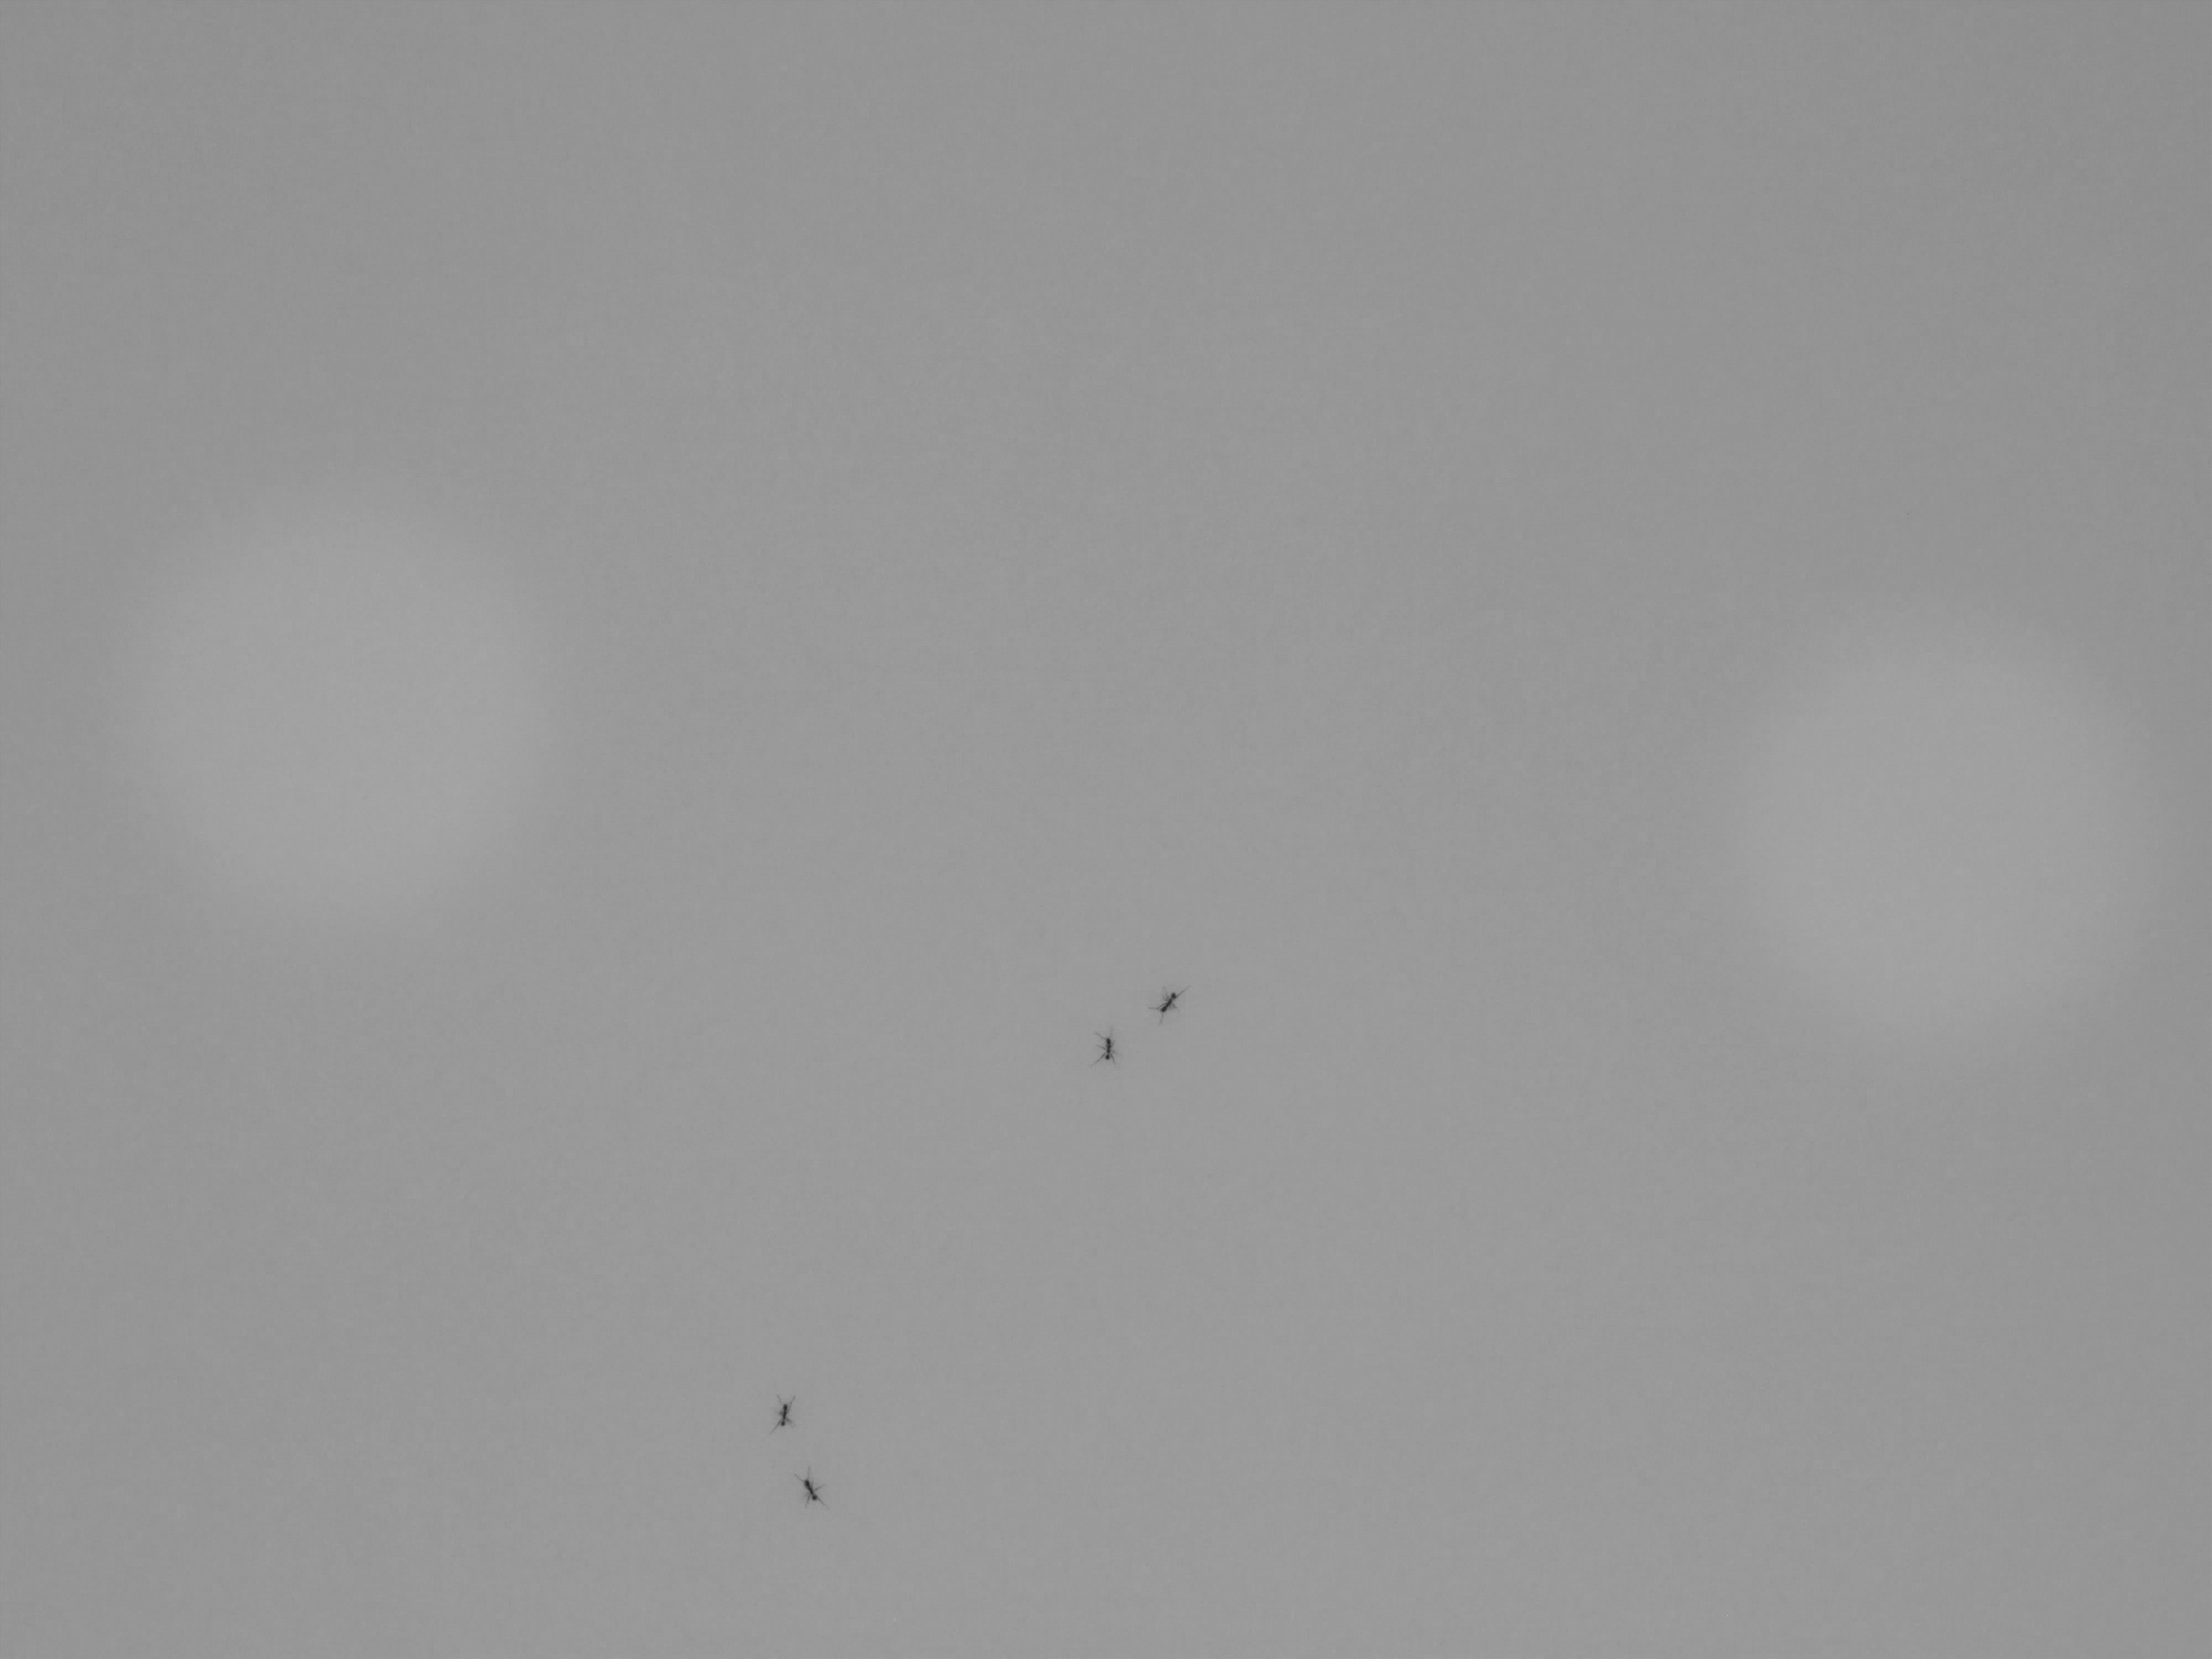
\includegraphics[width=\linewidth]{figures/05_methodology/initial_video_full.png}
        \caption[Frame from the initial video]{\footnotesize{A frame from the initial video.}}
        \label{fig:full frame initial video}
    \end{subfigure}
    \hspace{0.025\linewidth}
    \begin{subfigure}[b]{0.4\linewidth}
        \includegraphics[width=\linewidth]{figures/05_methodology/initial_video_ant.png}
        \caption[Zoom on frame from the initial video]{\footnotesize{A crop from the initial video.}}
        \label{fig:zoom frame initial video}
    \end{subfigure}
    \caption[Frame from the initial video setup]{\footnotesize{The Figure \ref{fig:zoom frame initial video} exposes the net on the upper layer of the Figure \ref{fig:full frame initial video}.}}
    \label{fig:frame initial video}
\end{figure}

\begin{figure}[!p]
    \centering
    \includegraphics[width=0.4\linewidth]{figures/05_methodology/second_video_full.png}
    \caption[Frame from the appearance video setup]{\footnotesize{A frame from one of the second set of videos.}}
    \label{fig:frame second video}
\end{figure}

\begin{figure}[!p]
    \centering
    \begin{subfigure}[b]{0.4\linewidth}
        \includegraphics[width=\linewidth]{figures/05_methodology/thirds_video_all.png}
        \caption[Frame from the more crowded tray video]{\footnotesize{A frame from the tray video with 87 ants.}}
        \label{fig:frame third video all}
    \end{subfigure}
    \hspace{0.025\linewidth}
    \begin{subfigure}[b]{0.4\linewidth}
        \includegraphics[width=\linewidth]{figures/05_methodology/thirds_video_set.png}
        \caption[Frame from the less crowded tray video]{\footnotesize{A frame from the tray video with 46 ants.}}
        \label{fig:frame third video set}
    \end{subfigure}
    \caption[Frames from the tray videos setup]{\footnotesize{Frames from the tray videos setup.}}
    \label{fig:frame third video}
\end{figure}

\FloatBarrier

\paragraph{MOT Challenge Format}

{
    To make the collected data useful for the tracking system, it must undergo a labeling process. 
    The main annotation format that was used is the \textbf{\ac{MOT} Challenge format}\cite{MOTChallenge2015}, 
    which is well-suited for both object tracking and object detection in videos. 
    This format is implemented as a \ac{CSV} text file per video with each line containing 10 fields: 
}

\begin{center}
    {``Frame, Id, left, top, width, height, confidence, 3D-World x, 3D-World y, 3D-World z"}
\end{center}

{
    In the case of 2D data, the 3D-World values are set to -1 and, in the case of detections, the Id value is also set to -1.
}

%\begin{table}[!h]
%    \centering
%    \caption[MOT Challenge format]{ \footnotesize MOT Challenge format with default values.}
%    \label{tab:MOT Challenge format}
%
%    \begin{tabularx}{\textwidth}{@{\hspace{1em}}Xl@{\hspace{1em}}|@{\hspace{1em}}X@{\hspace{1em}}X@{\hspace{1em}}}
%        \toprule
%        \textbf{Column} & \textbf{Field Name} & \textbf{Detection} & \textbf{Tracking} \\
%        \midrule
%        \midrule
%        1 & Frame number & \textless frame\textgreater & \textless frame\textgreater \\
%        2 & Identity number & -1 & \textless id\textgreater \\
%        3 & Detection left & \textless bb\_left\textgreater & \textless bb\_left\textgreater \\
%        4 & Detection top & \textless bb\_top\textgreater & \textless bb\_top\textgreater \\
%        5 & Detection width & \textless bb\_width\textgreater & \textless bb\_width\textgreater \\
%        6 & Detection height & \textless bb\_height\textgreater & \textless bb\_height\textgreater \\ 
%        7 & Detection confidence & \textless conf\textgreater & \textless conf\textgreater \\
%        8 & 3D World x & -1 & -1 \\
%        9 & 3D World y & -1 & -1 \\
%        10 & 3D World z & -1 & -1 \\
%        \bottomrule
%    \end{tabularx}
%
%\end{table}


{
    In addition to the main \ac{MOT} format, this project employs various dataset formats to simplify the training and deployment of different models. 
    These formats include the \ac{YOLO} dataset format\cite{yoloFormat} for image object detection, 
    the Market-1501 dataset format\cite{Market-1501} for appearance modeling, 
    and a custom format tailored for segmenting valid frames and IDs from the appearance videos.
}

\paragraph{YOLO Format}

{
    The \ac{YOLO} format is utilized for labeling single images extracted from videos. 
    Each image is associated with an equally named \ac{CSV} text-file that contains the following column fields for each detection:
}

\begin{center}
    {``class id, x-axis center, y-axis center, width, height"}
\end{center}

{
    It's important to note that the image fields are normalized based on the image shape. 
    Additionally, the \ac{YOLO} format defines a specific folder structure that separates images and labels into subfolders stemming from the same root. 
    A YAML file is used to describe the data paths and class indexes for each dataset.
}

{
    A tool was developed to convert the videos with a MOT Challenge annotations into images with a valid \ac{YOLO} format dataset. 
    This tool offers the flexibility to crop images (and the corresponding labels) into different segments, ensuring that each segment contains at least one whole ant in a random position. 
    The cropping feature maximizing the number of whole ants within each crop while guaranteeing that each ant is fully visible in at least one crop.
    Figure \ref{fig:yolo crop} shows an example of the results of this tool on a video.
}

\begin{figure}[!b]
    \centering
    \includegraphics[width=0.4\linewidth]{figures/05_methodology/yolo_crop.png}
    \caption[YOLO dataset: crop of 640x640 px]{\footnotesize{A crop of 640x640 px generated from an annotated video to create a YOLO Dataset.}}
    \label{fig:yolo crop}
    \vspace{-3em}
\end{figure}

\FloatBarrier

\begin{figure}[!htp]
    \centering
    \begin{subfigure}[b]{0.4\linewidth}
        \includegraphics[width=\linewidth]{figures/05_methodology/Market_unoriented.png}
        \caption[Samples of the unoriented appearance dataset]{\footnotesize{35 samples of the unoriented appearance dataset.}}
        \label{fig:unoriented appearance}
    \end{subfigure}
    \hspace{0.025\linewidth}
    \begin{subfigure}[b]{0.4\linewidth}
        \includegraphics[width=\linewidth]{figures/05_methodology/Market_oriented.png}
        \caption[Samples of the oriented appearance dataset]{\footnotesize{35 samples of the oriented appearance dataset.}}
        \label{fig:oriented appearance}
    \end{subfigure}
    \caption[Samples of the appearance datasets]{\footnotesize{Comparison between the output of the oriented and unoriented versions of the appearance dataset generation tools.}}
    \label{fig:appearance dataset}
    \vspace{-1.5em}
\end{figure}

\paragraph{Market-1501 Format}

{
    Market-1501 is a widely-used reidentification dataset organized based on folder and filename structures. 
    In this project, we mimic this format to simplify the deployment of the appearance model training, we call it Market-1501 Format.
}

{
    In Market-1501 Format, each ``ground truth detection" is cropped from the video and saved as an image within one of three folders: train, test, or test query. 
    and contains its identity on the filename. The identity of each detection is encoded in the filename.
}

{
    To convert the videos with MOT Challenge annotations into a Market-1501 dataset, a pair of tools were developed. 
    The first tool generates square crops using one of three strategies: 
    ``cropping and padding", ``cropping, padding the small size, and reshaping", or ``cropping and reshaping".
    The second tool generates rectangular crops with the head of the ant pointing downwards; 
    the shape of the crop is adjusted using similar methods to those employed by the first tool, 
    with the "padding the small size" option in the second tool being replaced by "padding to obtain the correct aspect ratio."
}

{
    The process of orienting the head of the ant downwards involves four steps:
}

\enlargethispage{1.5\baselineskip}

\begin{enumerate}
    \item The segmentation of the cropped ant by thresholding\footnote{Thresholding (neologism): Act of splitting a set of values using a threshold value.} the luminance level of the image.
    \item The computation of the direction of the body of the ant through principal component analysis.
    \item Determining the movement direction of the ant by comparing the current frame position with the nearest frame were the ants appears (if it is a previous frame, the origin point is the previous frame).
    \item Selecting the body direction of the ant that minimize the angular difference with the movement direction.
\end{enumerate}

\needspace{0.2\textheight}

{
    Figure \ref{fig:appearance dataset} provides an example of the output from each tool. 
    In both cases, padding was applied to one side before reshaping the crop.
    While there is an improvement, it's worth noting that the orientation solution in Figure \ref{fig:oriented appearance} has some limitations, 
    with a total of 35 instances, including 17 correct cases, 15 upside-down cases, and 3 instances with incorrect orientation.
}

\FloatBarrier

\paragraph{Custom Format}

{
    The custom format for segmenting video fragments is structured as a \ac{TSV} file with three columns. 
    The first column indicates the initial frame number, 
    the second column indicates the final frame number, 
    and the last column comprises a Python-styled list of lists that represents the invalid intervals. 
    These intervals are encoded by specifying their initial and final frames.
}

{
    Labeling is a time-consuming task that necessitates human supervision. 
    To reduce the time required, we employed an existing application and developed three additional tools.  
    The research on data annotation was conducted concurrently with the creation of a tutorial designed to guide the annotation of new training videos, which was one of the project's objectives.
}

\needspace{0.2\textheight}

\subsubsection{CVAT}

{
    \ac{CVAT}\cite{cvat} is an interactive annotation tool designed for computer vision applications. 
    It provides support for importing and exporting annotations in various popular formats. 
    In this project, we primarily relied on tracking results for labeling to save time on the annotation process.
}

{
    To set up \ac{CVAT}, it should be installed as a server through their Docker image and accessed through any web browser. 
    Figure \ref{fig:CVAT} shows the annotation interface.
}

{
    \ac{CVAT} manage each id as a class. 
    Within a frame, it offers functionalities to create, delete, and modify detections. 
    Additionally, any track can be created, deleted, marked as finished, split, merged, or have its identity changed.
    For unfinished tracks with gaps in the annotations, \ac{CVAT} employs linear interpolation, which can be adjusted manually in the desired frames.
}

{
    One limitation of \ac{CVAT} is that it supports a maximum resolution of 3000x2000 pixels.  
    To work around this, we utilized ffmpeg\cite{tomar2006converting} to downsample the video file and developed two scripts to adapt the annotations accordingly. 
    The commands in Listing \ref{lst:cvat_input} are used to generate the input video and importable annotations.
}

\begin{footnotesize}
    \begin{bashcode}[float=h, label={lst:cvat_input}, language=bash, caption={Commands to obtain the CVAT compatible data}]
        ffmpeg -y -i input.mp4 -vf scale=2000:-2,setsar=1:1 -c:v libx264 "input_downsampled.mp4"
        python3 minimum_id.py input_1.txt input_2.txt
        python3 prde_to_cvat.py input_2.txt output.zip
    \end{bashcode}
\end{footnotesize}

{
    A script was also created to convert manually corrected but downsampled annotations into the desired resolution.
}

{
    Despite the availability of preannotations from tracking models and the utility of this tool, 
    annotating 1375 frames (equivalent to approximately 1 hour and 30 minutes of video) still requires around 2 hours.
}

\begin{figure}[!tp]
    \centering
    \includegraphics[width=0.7\linewidth]{figures/05_methodology/CVAT.png}
    \caption[CVAT interface]{\footnotesize{A screenshot of the CVAT interface.}}
    \label{fig:CVAT}
\end{figure}

\subsubsection{Lonely Ant Frame Segmentation}

{
    In the process of generating video segment annotations from the collection of videos for appearance training, 
    a text file is filled manually with the previously listed specifications. 
    To speed up the process, a command that write the frame number on each frame using the ffmpeg tool is employed, as illustrated in Listing \ref{lst:frame_num_video}:
}

\begin{footnotesize}
    \begin{bashcode}[float=!h, label={lst:frame_num_video}, language=bash, caption={Command to write the frame number on each frame}]
        ffmpeg -i input.mp4 -vf "drawtext=fontfile=Arial.ttf: text=%{n}: fontsize=24: x=(w-tw)/2: y=h-(2*lh): fontcolor=white@0.5: box=1:boxcolor=0x00000099@0.3" -y input_frame_num.mp4
    \end{bashcode}
\end{footnotesize}
\FloatBarrier

{
    This approach reduces the time required for annotation to approximately 15 minutes for every hour of video footage. 
    Note that a video can be played at an accelerated speed, and this annotations only require pausing the video.
}

{
    Moreover, when dealing with sequences involving only one ant per frame and employing a high-performance detector, 
    this method becomes analogous to annotating in the MOT Challenge format. 
    By utilizing \textbf{detection by tracking}, the detector can effectively allow the low-confidence detections\footnote{This improves the detection recall, recall is a metric that will be explained in the following subsection about metrics.} and utilize a tracker to eliminate false positives.
    Even if the detector does not eliminate all the false positives, 
    adhering to the strict criterion of one ant per frame enables the initial exclusion of frames featuring multiple ants, 
    which can subsequently be interpolated as required.
}

\subsubsection{Purging by Deletion}

{
    A reliable object detector relies on a clean object detection dataset. 
    Given the impracticality on annotating with \ac{CVAT}, a different approach to create a object detection dataset was designed.
    This process utilized the script previously explained for generating a cropped (or uncropped) YOLO dataset, as illustrated in Figure \ref{fig:yolo crop}.
    To accomplish this, two additional scripts were developed.
}

{
    The initial step involves generating the object detection dataset using the YOLO dataset script. 
    The image filenames are assigned based on the frame IDs 
    (if no cropping was applied, it can be easily transformed into the MOT format).
}

{
    Next, the second script comes into play, which annotates the images and saves them in a new folder. 
    In cases where only one detection exists, a crop is retained, as it simplifies the process of assessing its accuracy via a file explorer. 
}

{
    Subsequently, annotators are tasked with deleting the invalid images from this folder.
}

{
    In the final step, a script is employed to construct a new dataset by copying only the remaining images. 
    This results in an object detection dataset where only a fraction of the frames are preserved, 
    typically less than half of the images prove to be valid.
}

{
    As an example, 50 seconds (equivalent to 750 frames) are transformed into 13,000 crops, 
    equivalent to a duration of approximately 14 minutes and 27 seconds. 
    The annotation process for this sequence typically takes around 4 hours to complete.
}

\subsubsection{Cleaning by Crop Deletion}

{
    While discarding images containing errors is an acceptable practice for object detection datasets, the aim is often to maximize available data. 
    To address this, we implemented another set of scripts, similar to the ones described previously.
}

{
    In this scenario, the data is initially in MOT format both at the beginning and the end of the process. 
    The first script is designed to store cropped images alongside their corresponding frame IDs and line numbers.  
    This script can source data from either one or two models. 
    In cases involving two models, it combines their outputs and attempts to identify true positives (which can be reviewed more swiftly), false positives, and false negatives.  
}

{
    The second script generates a MOT format file containing only the remaining lines, meaning that annotations for frames are corrected rather than deleted.
}

{
    In this case, cleaning 1 hour of video containing a single ant (equivalent to 54,000 frames) can be accomplished in roughly 6 hours. 
    This process was applied to 9 out of the 12 individual ant videos.
}

\needspace{0.2\textheight}

\subsubsection{Labeling strategies summary}

{
    The following table shows the speed of each strategy:
}

\begin{table}[H]
    \centering
    \caption[Labeling strategies speed]{ \footnotesize Labeling strategies speed }
    \label{tab:labeling speed}

    \begin{tabularx}{0.7\textwidth}{
        @{\hspace{0.05\textwidth}}
        >{\raggedright\arraybackslash}X
        >{\raggedleft\arraybackslash}X
        @{\hspace{0.05\textwidth}}
    }
        \toprule
        \textbf{Strategy} & \textbf{Speed} \\
        \midrule
        \midrule
        CVAT & 0.2 fps \\
        Lonely ant frames & 60 fps \\
        Purging by deletion & 0.9 fps \\
        Cleaning by deletion & 2.5 fps \\
        \bottomrule
    \end{tabularx}
\end{table}

\FloatBarrier

\needspace{0.25\textheight}
\subsection{Metrics}


{
    In the development of any engineering system, a fundamental aspect is the measurement of its performance. 
    In this project, we have one primary system, the \ac{MOT} tracker, along with two subsystems: the object detector and the appearance model. 
    Each of these components has its own set of evaluation metrics to quantify its performance
}

\subsubsection{Object Detection Metrics}

{
    An object detector solves the object localization and classification problems at the same time. 
    This kind of problem is evaluated by the precision, recall, F1-Score and \ac{mAP} metrics.
}

{
    These metrics require the definition of true positives, false positives and false negatives:
}

\begin{itemize}
    \item The \textbf{true positives} (\acs{TP}) are defined by correctly matching a class detections with ground truth objects of the same class. Usually a \ac{IoU} threshold is used to match the detections, similar to the association step of a SORT tracker.
    \item The \textbf{false positives} (\acs{FP}) are defined by incorrectly assigning a class on the detected object, it applies to matched objects and detected background.
    \item The \textbf{false negatives} (\acs{FN}) are defined by the absence of matching detections for ground truth objects.
\end{itemize}

\paragraph{Precision}

{
    Precision is a metric that measures the correctness of the detected set, a high precision means a high certainty on the detected objects, however it does not contemplate undetected objects.
}

\paragraph{Recall}

{
    Recall is a metric that measures the ability to detect targets, a high recall means a high certainty on detecting the relevant objects, however it does not contemplate undesired detections.
}

%\begin{figure}[!ht]
%    \centering
%    \includegraphics[width=0.3\linewidth]{figures/05_methodology/Precisionrecall.png}
%    \caption[Precision and recall]{\footnotesize{Visual representation of precision and recall extracted from WikipediaCommons\cite{precision_recall}.}}
%    \label{fig:precision and recall}
%\end{figure}
%
%{
%    Figure \ref{fig:precision and recall} describes graphically and mathematically precision and recall.
%}

\paragraph{F1-Score}

{
    F1-Score is the harmonic mean of precision and recall which symmetrically represents both metrics, it allows a good global evaluation of a model. 
%    Its formula is the following:
}

%\begin{equation}
%    \label{eqn:F1Score}
%    F_{1} = 2 \cdot \frac{precision \cdot recall}{precision + recall}
%\end{equation}

%{
%    Usually, deep learning based detection models return their confidence score. 
%    F1-Score, precision and recall computed on a validation dataset can be used to determine that parameter.
%    There is a compromise between precision and recall that makes the choice of a good threshold a non-trivial task.
%}

\paragraph{Mean Average Precision}

{
    \ac{AP} and \acl{mAP} (\ac{mAP}) are other global performance metrics like F1-Score. 
    \ac{AP} join precision and recall regardless of the confidence threshold for a given class. 
    \Ac{mAP} averages the \ac{AP} metric across multiple outputs generated by various user-defined settings. 
    These sets of outputs are referred to as queries.
}

{
    The most popular conventions for the \ac{mAP} set of settings are the isolation of each class and the definition of multiple \ac{IoU} threshold used to match the detections with the ground truth. 
    This project only detects one class, which means that only the \ac{IoU} threshold is modified.
}

%{
%    The \ac{AP} metric is obtained by averaging the precision curve ($P(R)$) in function of the recall ($R$) from 0 to 1:
%}

%\begin{equation}
%    \label{eqn:AP theory}
%    AP = \int_{0}^{1} P(R) \, dR
%\end{equation}

%{
%    In practice, the precision and recall curve is estimated by a given dataset becoming a set of not equidistributed points. 
%    In order to average the precision and recall curve, the data output is sorted by decreasing confidence (the $i-th$ detection is ranked $k_{i}$), the precision is computed within a subset of the $k$ more confident detections ($P(k)$) and, at the end, each ranked precision is weighted averaged by the width of the recall interval from the previous rank to the current rank.
%}

%\needspace{0.1\textheight}

{
%    The mathematical expression of the defined weighted average can be simplified into the simple mean of the ranked precision of the ground truth elements, with the false negatives redefined to have a ranked precision of 0:
    The \ac{AP} metric is obtained by averaging the precision in function of the recall curve. In practice, an estimation is obtained by a weighted average that can be simplified into the simple mean of the ranked precision of the ground truth elements, with the false negatives redefined to have a ranked precision of 0:
}

\begin{equation}
    \label{eqn:AP real}
    AP = \frac{\mathlarger{\sum\limits_{i \in TP}} P(k_{i})}{|TP| + |FN|}
\end{equation}

{
    This project uses the \textbf{\ac{mAP}@50} (or \ac{AP}@50 because there is only one class) and the \textbf{\ac{mAP}@50-95}. 
    The @ notation refers to the \ac{IoU} threshold queries, being \textbf{\ac{mAP}@50} the \ac{AP} when the \ac{IoU} is set to 0.5 and \textbf{\ac{mAP}@50-95} the mean of the \ac{AP} computed with \ac{IoU} thresholds of 0.5, 0.55, 0.6, 0.65, 0.7, 0.75, 0.8, 0.85, 0.9 and 0.95.
}

\subsubsection{Identity Re-identification Metrics}

{
    An appearance model solves the identity re-identification problem. 
    This kind of problem is evaluated by the rank metrics and the already seen \textbf{\ac{mAP}} using the identities on the desired validation dataset classes as queries.
}

{
    In re-identification problems true negatives can also be defined, in addition to true positives, false positives and false negatives:
}

\begin{itemize}
    \item The \textbf{true positives} are defined by correctly matching pairs of ants images with the same identity.
    \item The \textbf{true negatives} (\acs{TN}) are defined by correctly not matching pairs of ants images with different identities.
    \item The \textbf{false positives} are defined by incorrectly matching pairs of ants images with different identities.
    \item The \textbf{false negatives} are defined by incorrectly not matching pairs of ants images with the same identities.
\end{itemize}

\paragraph{Rank metrics}

{
    The $k$-rank metrics redefine true positives (${TP}_{k}$) by the existence on any correct match for a query ant within the $k$ nearest appearances.
    The final metric is the accuracy of the given set of queries:
}

\begin{equation}
    \label{eqn:rank accuracy}
    Rank_{k} = \frac{|{TP}_{k}|}{|queries|}
\end{equation}

{
    This project contemplates the rank-1 metric or accuracy.
}

\needspace{0.15\textheight}

\subsubsection{Multiple Object Tracking Metrics}

{
    Evaluating multiple object tracking is a complex problem comparable to the tracking task itself. 
    The reason of this complexity is the fact that a tracking system solves 3 problems:
}

\begin{itemize}
    \item \textbf{Detection}: the target objects are found. % independently of the identity. but the matching score priorize identity to get TP anyway
    \item \textbf{Localization}: the found objects are spatially aligned with their target. % independently of the identity. but the matching score priorize identity to get TP anyway
    \item \textbf{Association}: the found objects are temporally aligned with their target identity.
\end{itemize}

{
    For this reason, there exist a lot of metrics that prioritize one problem over the others or evaluate each problem with different criteria.
    In this project, it was decided to use the \ac{HOTA}\cite{luiten2020IJCV} group of metrics because the authors of these metrics states that the \ac{HOTA} metric, that jointly evaluates the three problems, is balanced with respect the three problems (see Figure \ref{fig:hota_vs_others}).
}

\begin{figure}[!h]
    \centering
    \includegraphics[width=0.75\linewidth]{figures/05_methodology/HOTA_vs_other.png}
    \caption[HOTA compared with other metrics]{\footnotesize{
        Image extracted from the HOTA paper\cite{luiten2020IJCV}. \\
        HOTA, DetA and AssA compared with other popular metrics (MOTA\cite{MOTA} and IDF1\cite{ristani2016performance}).
        }}
    \label{fig:hota_vs_others}
\end{figure}

{
    Similar to the other metrics, the first step is the definition of true positives, false negatives and false positives. 
    However, to obtain these values, a matching between ground truth and tracks is required.
    This matching should aim to maximize the final metric while maintaining plausibility. 
    The rationale behind this criterion is that all consistent interpretations of the system's output that align with the ground truth are valid, 
    and the maximized interpretation is likely the most accurate.
}

{
    The authors of \ac{HOTA} solve this optimization problem with the Hungarian algorithm using a composed score. The score uses a \textbf{current frame} spatial similarity component and a \textbf{global} estimated ``optimal association" score.
    The estimated association score is a prematching proxy for an association score that approaches the estimated one for the optimal assignment.
}

{
    The spatial similarity can be the previously explained \ac{IoU}, the previous ``plausibility'' refers to a threshold value applied on this score after the ground truth matching. 
}

{
    The estimated association score is a multiple frames Jaccard index\footnote{The Jaccard index is the intersection of two sets over their union (\ac{IoU}).}, it is computed as the available spatial associations (with a higher spatial similarity than the threshold) of a pair ``ground truth identity''-``tracked object identity'' for all the frames over the number of frames where at least one of the identities was present (see Figure \ref{fig:hota_preassociation}).
}

\begin{figure}[!h]
    \centering
    \includegraphics[width=\linewidth]{figures/05_methodology/HOTA_association_example.png}
    \caption[HOTA: Track overlap with ground truth]{\footnotesize{
        This image illustrates a case where a track of 3 frames overlaps during 2 frames with a ground truth identity of 4 frames. 
        The denominator of the estimated optimal association will be 3-2+4=5. 
        The numerator can be 2 for a threshold smaller than 0.5, 1 for a threshold smaller than 0.8 and 0 for a threshold higher than 0.8. 
        With a threshold of 1 the association score cannot be different than the estimated association score.
        }}
    \label{fig:hota_preassociation}
\end{figure}

{
    Once the spatial similarity ($\mathcal{S}$), the estimated association score ($\mathcal{A}_{max}$) and the similarity threshold ($\alpha$) are defined, the potential matching score used for the linear assignment joins them as in the equation \ref{eqn:potential matching score}:
}

\begin{equation}
    \label{eqn:potential matching score}
    MS(i, j) = \begin{cases}
        \frac{1}{\varepsilon} + \mathcal{A}_{max}(i, j) + \varepsilon \cdot \mathcal{S}(i, j) & \text{if } \mathcal{S}(i, j) \geq \alpha\\
        0 & \text{otherwise}
    \end{cases}
\end{equation}
    
{
    The matching algorithm was implemented in order to use the ground truth to analyses our results and test the viability of a model.
}

{
    With a mapping between ground truth and output tracks, \ac{HOTA} defines true positives, false negatives, false positives:
}

\begin{itemize}
    \item The \textbf{true positives} are detections that are matched with a ground truth object, independently of the identity, it measures the performance of the detection and localization problems.
    \item The \textbf{false negatives} are ground truth objects that are not matched.
    \item The \textbf{false positives} are detections that are not matched.
\end{itemize}

{
    Additionally, \ac{HOTA} defines new values called true positives associations (\acs{TPA}), false negatives associations (\acs{FNA}) and false positives associations (\acs{FPA}).
    The \ac{TPA}, \ac{FNA} and \ac{FPA} are defined independently over all the pairs of ``ground truth identity''-``tracked object identity'' within the true positives set; a single evaluation has got one set of true positives, false negatives and false positives and $C=|TP|$ sets of true positives associations, false negatives associations and false positives associations. 
    These values measure the performance of the association problem:
}
\begin{samepage}
    \begin{itemize}
        \item The \textbf{true positives associations}, given a true positive of interest ``c", are all the true positives which have the same ``ground truth identity''-``tracked object identity'' pairs than the interest true positive ``c"; all \ac{TPA}s have the same \ac{TPA}, \ac{FNA} and \ac{FPA} which reduce the number of computation although the concept is defined for all the \ac{TP}s.
        \item The \textbf{false negatives associations}, given a true positive of interest ``c", are the ground truth objects with the same identity as the ground truth from ``c'' that were not assigned the tracked object identity from ``c'' (different or unassigned identities).
        \item The \textbf{false positives associations}, given a true positive of interest ``c", are the detections with the same identity as the detection from ``c'' that were not assigned the ground truth identity from ``c'' (different or unassigned identities).
    \end{itemize}
\end{samepage}

{
    With the new association measures, the previously mentioned association score can be properly defined:
}

\begin{equation}
    \label{eqn:association score}
    \mathcal{A}(C) = \frac{|TPA(c)|}{|TPA(c)| + |FNA(c)| + |FPA(c)|}
\end{equation}

\paragraph{\ac{HOTA}\textsubscript{$\alpha$}}

{
    \ac{HOTA}\textsubscript{$\alpha$} is a metric defined by a double Jaccard formulation, where the association score ($\mathcal{A}$) is a Jaccard metric over the associations that weights the true positives of a Jaccard metric over the detection concept. 
    And $\alpha$ is the threshold on location similarity.
}

\begin{equation}
    \label{eqn:hota alpha}
    HOTA_{\alpha} = \sqrt{\frac{\sum_{c \in \{TP\}} \mathcal{A}(c)}{|TP| + |FN| + |FP|}}
\end{equation}

{
    The square root is needed because the dimensionality of the summation of association scores (multiplied by true positive of value 1) is squared (jointly detection domain and association domain) over unsquared (association domain), and the detection Jaccard makes the denominator squared (jointly detection domain and association domain).
}

\paragraph{\ac{HOTA}}

{
    Theoretically, \ac{HOTA} is the average of $HOTA_{\alpha}$ on all the location similarity domain (from 0 to 1). In practice, it can be approximated by a mean:
}

\begin{equation}
    \label{eqn:hota}
    \text{HOTA} = \int_{0}^{1} \text{HOTA}_{\alpha} \, d\alpha \approx \frac{1}{19} \cdot \sum_{\alpha \, \in \, \{0.05 \cdot i \,|\, 1 \leq i \leq 19\}} \text{HOTA}_{\alpha}
\end{equation}

\paragraph{LocA}

{
    Localization Accuracy (\ac{LocA}) is a measure of localization that average the different localization thresholds:
}

\begin{equation}
    \label{eqn:loca}
    \text{LocA} = \int_{0}^{1} \frac{1}{|\text{TP}_{\alpha}|} \cdot \sum_{c \, \in \, \{\text{TP}_{\alpha}\}} \mathcal{S}(c) \, d\alpha
\end{equation}

\paragraph{DetA}

{
    Detection Accuracy (\ac{DetA}) is the detection Jaccard index with a given localization threshold $\alpha$. It can be further decomposed into detection precision and detection recall but it is not used in this project.
}

\begin{equation}
    \label{eqn:deta}
    \text{DetA}_{\alpha} = \frac{|\text{TP}_{\alpha}|}{|\text{TP}_{\alpha}| + |\text{FN}_{\alpha}| + |\text{FP}_{\alpha}|}
\end{equation}

\paragraph{AssA}

{
    Association Accuracy (\ac{AssA}) is a measure of association that average the association score with a given localization threshold $\alpha$.
}

\begin{equation}
    \label{eqn:assa}
    \text{AssA}_{\alpha} = \frac{1}{|\text{TP}_{\alpha}|} \cdot \sum_{c \, \in \, \{\text{TP}_{\alpha}\}} \mathcal{A}(c) \, d\alpha
\end{equation}

{
    Another interpretation of \ac{HOTA}\textsubscript{$\alpha$} is the geometric mean of \ac{DetA}\textsubscript{$\alpha$} and \ac{AssA}\textsubscript{$\alpha$}.
}


\needspace{0.25\textheight}
\subsection{Detection Models}


{
    To facilitate the development of multiple detection models and their subsequent integration into the tracker, we designed a versatile program. 
    This program processes input videos and saves the output detections in a MOT format file with an easily replaceable detector. 
}

%\begin{figure}[!p]
%    \centering
%    \includegraphics[width=0.6\linewidth]{figures/05_methodology/DetectionScript.png}
%    \caption[Generic detection script]{\footnotesize{
%            Block diagram of the detection script.
%        }}
%    \label{fig:DetectionScript}
%\end{figure}

{
    Initially, there was no labeled data to train any data-driven model, for this reason, the first implemented model was a deductive model.
}

{
    This deductive model, as the examples from the tracking software subsection of the state of the art, is based on background extraction.
}

{
    To ensure accurate background estimation, this model requires a set of training frames. 
    The estimation is performed using a Gaussian Mixture-based model, which becomes reliable after proper training. 
    In this project, 500 frames were used because the input videos allowed it, however, with 50 frames is enough.
}

{
    Once the background is estimated, it is subtracted from the frame to isolate the foreground. 
    A morphological filter consisting in a 5x5 closure to reduce noise inside the ant body, 
    followed by a 3x3 opening is then applied to the foreground to reduce noise in the background estiamtion. 
    The remaining connected components with a minimum pixel count are identified as the output detections.
}

%\begin{figure}[!h]
%    \centering
%    \includegraphics[width=0.6\linewidth]{figures/05_methodology/fgbg_code.png}
%    \caption[Background extraction detection model block diagram]{\footnotesize{
%            Block diagram of the background extraction based model.
%        }}
%    \label{fig:fgbg_code}
%\end{figure}

\FloatBarrier

{
    With the first detection model results, filtered by a tracker and corrected with the developed annotation tools, a initial dataset was created; it was used to train a deep learning model.
    After some iterations of training, detection of new data and cleaning, the final dataset used for detection training was created. 
    The test was performed on an unseen set of data manually annotated: a video fragment which can represent the final deployment.
    The first video was excluded.
}

{
    The following table contains the training, validation and test splits:
}

\begin{table}[H]
    \centering
    \caption[Detection dataset size]{ \footnotesize Detection dataset size.}
    \label{tab:detection splits}

    \begin{tabular}{p{3cm} rr}
        \toprule
        \textbf{Subset} & \textbf{Images} & \textbf{Percentage} \\
        \midrule
        \midrule
        \textbf{Training} & 8374 & 68.7\% \\
        \textbf{validation} & 3662 & 30.1\% \\
        \textbf{Test} & 150 & 1.2\% \\
        \bottomrule
    \end{tabular}
\end{table}

{
    The deep learning model selected for this project is the Ultralytics\cite{Jocher_YOLO_by_Ultralytics_2023} library \ac{YOLOv8} architecture \ac{YOLOv8n} model (detailed in the state of the art section).
    The decision to opt for this architecture was based on state of the art performance in popular challenges as well as simplicity of training and inference deploying (Ultralytics implements most of the standard training features).
}

{
    The choice of model was based on the current problem, the ants on the frames are small objects, and it has two main consequences: 
}

\begin{itemize}
    \item Deep neural networks tend to reduce the spatial dimension while expanding the feature dimension; this means that the ant location becomes uncertain.
    \item Deep neural networks requires a fixed input size, if the input is large, the training may suffer from lack of memory; however, if the input is resized into a smaller size, the small ants may disappear.
\end{itemize}

{
    A slicing windows analysis was deployed in order to solve this issues.
    For the training, 640x640 px crops were used; and, for the inference, a slicing windows was applied using the \ac{SAHI} library\cite{Akyon_Slicing_Aided_Hyper_2022,obss2021sahi}. 
    This method divides the image into a set of overlapped sub-images without any reshaping. 
    However, it results in longer training and inference times, as each image is transformed into multiple sub-images.
}

{
    Additionally, \ac{YOLOv8n}, the smallest \ac{YOLOv8} model, was selected by experimentation.
}

\needspace{0.2\textheight}

\subsubsection{YOLOv8 Training}

{
    Ultralytics is fully integrated with \ac{WandB}\cite{wandb}, a machine learning development platform that helps in the real-time tracking and visualization of experiments, it also have an automatized launcher for hyperparameter sweeping. 
    Using \ac{WandB} resources to visualize enough trainings, the lower and upper thresholds of each available hyperparameter were adjusted until the setting in Table \ref{tab:detection hyperparameters}.
}

\begin{table}[H]
    \centering
    \caption[Detection Model hyperparameters]{ \footnotesize Detection Model hyperparameters.}
    \label{tab:detection hyperparameters}

    \begin{tabularx}{0.9\textwidth}{
        @{\hspace{0.025\textwidth}}
        >{\raggedright\arraybackslash}X
        >{\raggedleft\arraybackslash}X
        @{\hspace{0.025\textwidth}}
    }
        \toprule
        \textbf{Hyperparameter Name} & \textbf{Values} \\
        \midrule
        \midrule
        Hue (maximum deviation) & min=0, max=0.3\\
        Saturation (maximum deviation) & min=0, max=0.5\\
        Value (maximum deviation) & min=0, max=0.5\\
        Rotation (maximum degrees) & min=60º, max=180º\\
        Translation (fraction of input) & min=0, max=0.5\\
        Scale (maximum gain and loss) & min=0, max=1\\
        Flip upside down (probability) & min=0, max=0.5\\
        Flip left-right (probability) & min=0, max=0.5\\
        Mosaic (probability) & min=0, max=1\\
        Shear (maximum degrees) & min=0, max=15\\
        Perspective (fraction) & min=0, max=0.001\\
        Mixup (probability) & min=0, max=0.12\\
        Copy paste (probability) & min=0, max=1\\
        \midrule
        Dropout & \{0, 0.25, 0.5, 0.75\} \\
        \midrule
        Batch size & min=50, max=100 \\
        Optimizer & \{SGD, AdaM\} \\
        Initial learning rate & min=0.001, max=0.01 \\
        Final learning rate & min=0.0001, max=0.001 \\
        Warmup epochs & 10 \\
        Cosine learning rate & \{True, False\} \\
        Momentum & min=0.9, max=0.974 \\
        \midrule
        Maximum epochs & 500 \\
        Early stopping patience & 50 epochs \\
        \midrule
        NMS & \{Agnostic, False\}\\
        NMS IoU & min=0.5, max=1\\
        \bottomrule
    \end{tabularx}
\end{table}

%\needspace{0.25\textheight}

{
    The first group of hyperparameters refer to the data augmentation used to help the model generalize better with the same amount of data, as each time a imaged is loaded, it will be randomly modified within a certain limits. 
    It includes modification in the images coloration, the appearance of the objects within the image, small modifications of the objects (a flip will create a symmetrical but inexistent ant) and some combination of various images. 
    Figure \ref{fig:detector_data_augmentated} shows a set of 16 images after data augmentation.
}

\begin{figure}[!tp]
    \centering
    \includegraphics[width=0.5\textwidth]{figures/05_methodology/TrainDataDetector.jpg}
    \caption[YOLOv8 data augmentated]{\footnotesize{Samples of the augmentated training data for the best detector trained.}}
    \label{fig:detector_data_augmentated}
\end{figure}

{
    The second group of hyperparameters refer to the model, in this case, there is only the dropout; it randomly set to zero certain values in the mathematical expression of a forward pass to reduce the number of useless nodes as well as generalize by randomizing.
}

{
    The third group of hyperparameters refer to the weight upgrading to reach an optimum result on the loss function.
    The loss function for these trainings is a combination of binary cross entropy and focal loss for classification (with only one class, ant, both of them are equivalent) and a mean squared error (\ac{MSE}) for the object location.
    The hyperparameters include the number of images used as a representative sample of the world that the model should learn, how the model will find the best weights to fit the current batch samples and the speed (with not a well-defined meaning) at which it will try to reach that weights.
}

{
    The fourth group set a limit on how long it should take to reach the limit, and the maximum steps admissible without validation improvement.
}

{
    The last group is about post-processing the outputs, only the suppression of highly overlapped detections is contemplated.
}

{
    At the end, the best models were selected, added to the detection script with \ac{SAHI} and their outputs were used in the tracker.
}


\needspace{0.25\textheight}
\subsection{Appearance Model}


{
    Similar to the detection model, the first step was the development of a script that applies the appearance model. 
    In this case, the script takes a MOT format file and its video.
    It applies the appearance model on each line of the MOT file.
    And the output is the input MOT file with each line extended with as many columns as appearance features returns the model.
}

{
    For the appearance model, the choice of model was directly obtained from Deep OC-SORT (a model from 2023): the Bag of Tricks model\cite{Luo_2019_CVPR_Workshops}. 
    The rationale behind this choice was twofold: 
    first, given the limited availability of appearance data, there were modest expectations for its performance in the initial video. 
    Second, Deep OC-SORT represents a state-of-the-art model, further justifying its selection.
}

{
    The implementation of this model is the same from Deep OC-SORT, it is the model from the FastReID\cite{he2020fastreid} library which includes training scripts. 
    In this case, a tuning of the FastReID source code was needed. The inference function was extracted from the Deep OC-SORT code and applied on the developed inference scripts.
}

\subsubsection{Bag of Tricks Training}

{
    Being a relatively simple model architecture (detailed in the state of the art section), 
    the more relevant part of this model is the training, more specifically, the training tricks defined on their paper and code:
}

\begin{itemize}
    \item The triplet loss, a derivable function for maximizing interclass euclidean distance and minimizing intraclass euclidean distance, is applied before the batch normalization layer.
    \item The classification loss is still derivated from the output of the pooling layer.
    \item The first 1000 iterations from a total of 18000 has the backbone freezed.
    \item The first 2000 iterations are warm-up iterations and the learning rate increases.
    \item From the iteration 2000 until the iteration 9000 the learning rate is constant.
    \item From the iteration 9000 until the end, the learning rate decrease with a cosine decay.
\end{itemize}

{
    The implementation used for training is the same of the paper, with the only difference in the data augmentation: the code was modified in order to allow the definition of rotation degrees and the use of rotation without any additional affine transformations. 
    Most of the training options were reduced based on the paper.
}

{
    The biggest ant appearance dataset that was used contained 186 identities, divided into 93 for training and 93 for validating. 
    The validation set will leave a 20\% of the identities as unknown identities (these identities are true negatives). 
    At the end, the train set has got 6730 images, the validation query set has got 489 images to assign in 5795 images. 
}

{
    The model was not tested using the criteria from the training. 
    Nevertheless, a custom set of tests, that will be explained in the following subsection, 
    were performed on an unseen set of data manually annotated: a video fragment with 87 simultaneous identities which represent the worst case scenario.
}

\enlargethispage{1.5\baselineskip}

\needspace{0.1\textheight}

{
    The following table summarize the data splits:
}

\begin{table}[H]
    \centering
    \caption[Appearance dataset size]{ \footnotesize Appearance dataset size.}
    \label{tab:appearance splits}

    \begin{tabular}{p{3cm}l rrr}
        \toprule
        \multicolumn{2}{c}{\textbf{Subset}} & \textbf{Identities} & \textbf{Images} & \textbf{Percentage} \\
        \midrule
        \midrule
        \multicolumn{2}{l}{\textbf{Training}} & 93 & 6730 & 51.1\% \\
        \multirow{2}{*}{\textbf{Validation}} & Test images & 93 & 5795 & 44.0\% \\
        & Query identities & 74 & 489 & 3.7\% \\
        \multicolumn{2}{l}{\textbf{Test}} & 87 & 150 & 1.2\% \\
        \bottomrule
    \end{tabular}
\end{table}

\vspace{1\baselineskip}

{
    Additionally, a small script to allow the use of \ac{WandB} to visualize the experiments as a whole and lunch automatic sweeps was written. 
    The set of hyperparameter values that were allowed is defined in Table \ref{tab:appearance hyperparameters}.
}

\begin{table}[H]
    \centering
    \caption[Appearance Model hyperparameters]{ \footnotesize Appearance Model hyperparameters.}
    \label{tab:appearance hyperparameters}

    \begin{tabularx}{0.9\textwidth}{
        @{\hspace{0.025\textwidth}}
        >{\raggedright\arraybackslash}X
        >{\raggedleft\arraybackslash}X
        @{\hspace{0.025\textwidth}}
    }
        \toprule
        \textbf{Hyperparameter Name} & \textbf{Values} \\
        \midrule
        \midrule
        Augmentation mix (probability) & min=0, max=1\\
        Brightness (maximum deviation) & min=0, max=2\\
        Contrast (maximum deviation) & min=0, max=2\\
        Hue (maximum deviation) & min=0, max=0.5\\
        Saturation (maximum deviation) & min=0, max=2\\
        Flips 50\% enabled & \{True, False\}\\
        Rotation (maximum degrees) & min=60, max=100\\
        \midrule
        Batch size & 8192 \\
        Optimizer & \{SGD, AdaM\} \\
        Initial learning rate & min=0.00001, max=0.005 \\
        Momentum & min=0.9, max=0.95 \\
        \midrule
        Maximum epochs & 1440 \\
        \bottomrule
    \end{tabularx}
\end{table}

\vspace{1\baselineskip}

{
    To adjust the color mean and standard deviation, a script to analyze the pixels of a whole video was made.
}

{
    Finally, the unoriented and the oriented versions of the same dataset trained were trained. The best models independently of the dataset were used to perform a test of viability.
}

\needspace{0.1\textheight}

\subsubsection{Appearance Tests}

{
    As the training of the appearance features was unconvincing, in order to analyze the discriminability of appearance, a set of tests were designed.
}

{
    The first test consists in the comparison of ants with themselves rotated using different rotation angles and plotting the distance with respect the angular rotation, the goal of this test is the study of the invariance over rotation that a well trained appearance model should have.
}

{
    The second test is a comparison of ants with other ants rotated, this also checks the invariance over rotation but from the error point of view.
}

{
    The third test is the splitting of all tracks within a ground truth into tracklets every time two or more ants are near; afterwards, the mean appearance of the tracklets, the limit appearance near a split point and the re-joining capabilities were observed through a set of correct versus incorrect appearance distance histograms.
}


\needspace{0.25\textheight}
\subsection{Tracking Models} 


% Include PCA Model and data analysis

{
    For the tracking model development, a proxy detector that reads the output of the previous detection models or appearance model was used. It removes the time and memory needed for video loading and reduce the time used on redundant computations.
}

{
    The first model tested was a SORT model with a downgraded detector, the background extraction model (see Figure \ref{fig:fgbg_code}). 
    The next model tested was the OC-SORT model with the same the background extraction model as the model.\\
    The code from these trackers was reimplemented to gain understanding and flexibility to apply modifications.
}

{
    Afterwards, a manual annotation was performed to define the project baseline. 
    This annotated data allowed the analysis of the ants behavior, by instance, the displacement per frame, the time of potential occlusions, the location metrics distribution, etc. 
    It also allowed the study on the error distribution: the velocity and angular errors from the Kalman estimations.
}

{
    Before training the deep learning based detector, a test to improve the Kalman filter from the OC-SORT model with an intuition was developed. 
    The intuition consisted on ``the ants should move towards the direction their body points". 
    It was implemented by instantaneously modifying the direction of the estimation (less than 180º) using \ac{PCA} on the ants body. 
    %A study on the error distribution was performed and compared with the previous trackers results.
    To reduce the input loading time, the angle obtained through \ac{PCA} was included on the MOT file.
}

{
    With a better detector, the SORT and OC-SORT model were tested again.
}

{
    Finally, the Deep SORT model was reimplemented and the Deep OC-SORT github code was downloaded. These models were tested with the trained appearance model.
}

